\documentclass[11pt]{article}

\usepackage[letterpaper,margin=0.95in]{geometry}
\usepackage{amsmath,amssymb,mathtools}
\usepackage{booktabs}
\usepackage{enumitem}
\usepackage{graphicx}
\usepackage{hyperref}
\usepackage{microtype}
\usepackage{xcolor}
\usepackage{url}

\hypersetup{
  colorlinks=true,
  linkcolor=black,
  citecolor=blue!55!black,
  urlcolor=blue!55!black
}

\setlength{\parindent}{0pt}
\setlength{\parskip}{0.48em}
\setlist[itemize]{leftmargin=1.35em,itemsep=0.16em,topsep=0.18em}
\setlist[enumerate]{leftmargin=1.45em,itemsep=0.16em,topsep=0.18em}
\renewcommand{\arraystretch}{1.12}

\newcommand{\base}{\mathrm{b}}
\newcommand{\qasset}{\mathrm{q}}
\newcommand{\cash}{\mathrm{cash}}
\newcommand{\live}{\mathrm{live}}
\newcommand{\hlp}{\mathrm{hLP}}
\newcommand{\ylp}{\mathrm{yLP}}
\newcommand{\debt}{\mathrm{debt}}
\newcommand{\nad}{\mathrm{NAD}}
\newcommand{\bps}{\mathrm{bps}}
\newcommand{\ema}{\mathrm{EMA}}
\newcommand{\nav}{\mathrm{NAV}}

\title{\vspace{-1.6em}Omnipair Dusk: A Generalized Automated Market Maker for Oracle-less Lending and Leveraged Liquidity}
\author{
  Omnipair Contributors\\[-0.25em]
  \small Expanded technical draft for Omnipair Dusk v2\\[-0.25em]
  \small \url{https://github.com/omnipair}
}
\date{Draft, July 2026}

\begin{document}
\maketitle
\vspace{-1.2em}

\begin{abstract}
Omnipair Dusk is an oracle-less pair-local market on Solana. It combines constant-product exchange, isolated lending, yield-bearing LP shares, leveraged LP vaults, and isolated spot-margin leverage inside a single reserve accounting model. The central reserve coordinate is
\[
R_{\live,i}=R_{\cash,i}+D_{\cash\text{-}\debt,i}+R_{\hlp,i},
\]
where cash reserves, cash-backed debt, and hLP live depth are separate state variables. This equation gives ordinary borrowing price neutrality, gives swaps their usual constant-product behavior, and gives hLP a named synthetic depth coordinate rather than an implicit exception. The paper formalizes the Dusk market model, explains yLP and hLP accounting, describes isolated leverage and liquidation, and relates the design to Curve, Morpho, Yield Basis, and adjacent AMM-lending systems. It ends with deterministic simulations of adaptive interest rates, live-depth slippage, and hLP tracking loss. The objective is not to claim that every long-tail asset is safe to lever. It is to show how oracle-less markets can make risk local, explicit, and mechanically bounded.
\end{abstract}

\textbf{Disclaimer.} This document is for research and implementation review. It is not investment, legal, accounting, tax, or financial advice. Dusk v2 is experimental, unaudited, and under active development.

\section{Introduction and Motivation}

Decentralized exchange and decentralized credit are usually built as separate systems. An automated market maker holds inventory and quotes trades. A lending market holds collateral and debt. Liquidation bots or routers convert one into the other when a position becomes unhealthy. The separation is convenient for mature assets with deep markets and widely available oracle feeds. It is much less convincing for long-tail assets, where price feeds are sparse, liquidity moves quickly, and liquidation liquidity is often the same liquidity that originally established the price.

The user demand is large enough to matter. A public Omnipair notebook sampling the top 3000 Raydium pairs by 24-hour volume found that 78.41\% of sampled volume was in pairs below \$100M fully diluted valuation, and roughly 94.82\% was below \$1B \cite{omnipair-raydium-notebook}. The result should be interpreted carefully. It does not imply that low-FDV assets are good collateral. It only shows that meaningful trading activity lives outside the small set of assets that can be listed by conservative oracle-governed lending markets.

Dusk starts from the opposite direction: if the market itself is the best available price source, the lending system should not be external to that market. Omnipair's Generalized Automated Market Maker (GAMM) thesis is that a pair-local AMM can provide the spot coordinate, the borrowable inventory, and the liquidation route for that pair \cite{omnipair-docs-intro,omnipair-docs-gamm}. Liquidity providers deposit both assets. Traders swap against the same reserves. Borrowers post one side to borrow the other. Losses and constraints are local to the pair.

This paper expands that thesis for Dusk v2. The design retains the constant-product core, but adds three accounting layers that are intentionally separated:
\begin{enumerate}
  \item yLP, a normal two-sided LP share with yield distributed through fee and interest growth indexes;
  \item cash-backed debt, which removes cash but preserves the live reserve coordinate at borrow time;
  \item hLP, an aggregate 2x leveraged LP vault that adds explicit synthetic live depth and funding debt.
\end{enumerate}

The point of this separation is auditability. A cash balance is not a price coordinate. A price coordinate is not always withdrawable cash. A debt share is not an LP share. A live reserve can include synthetic hLP depth, but a token transfer can only spend cash. Dusk attempts to make these distinctions visible in the state transition algebra rather than recoverable only from implementation folklore.

The paper has two versions in this repository. The compact note is intended as a short research introduction. This expanded draft is intended for reviewers who want to see how the pieces compose: yLP accounting, hLP NAV, isolated spot-margin leverage, adaptive rates, risk references, and liquidation. The style follows recent protocol papers that define mechanism first and implementation after, rather than leading with product surface \cite{morpho-midnight}.

\subsection{Design Objectives}

Dusk is optimized for a different question than most lending protocols. The question is not "what is the correct external price of this asset?" The question is "what can this particular market safely recover, settle, and quote from its own state?" That shift gives the protocol five design objectives.

\textbf{Local solvency.} A market should be able to state its own assets, liabilities, and recovery path without depending on another market. Local solvency does not guarantee that every position can be made whole. It means deficits and buffers are pair-specific and visible.

\textbf{Price-through-liquidity.} A collateral valuation should degrade as position size approaches available depth. Linear marks are too generous for long-tail assets because liquidation itself moves the price. Dusk therefore uses AMM output functions in risk valuation.

\textbf{Explicit synthetic depth.} If the protocol wants synthetic live depth, it should name it. hLP depth is not hidden in cash reserves and not confused with cash-backed debt. It has its own vault owner, debt, NAV, and settlement constraints.

\textbf{O(1) aggregate accounting.} Swaps and rebalances cannot iterate over user positions. hLP is aggregate by construction, and yLP yield is checkpointed through indexes. The market can update global state without scanning all LPs or borrowers.

\textbf{Conservative liveness.} The market should keep ordinary swaps live when possible, even if hLP target state cannot be fully reached immediately. Pending rebalance is an example: it preserves the fact that a target remains unfinished without blocking all activity.

These objectives are sometimes in tension. Strict settlement guards can reduce liveness. More live depth improves execution but can increase complexity around cash headroom. More adaptive rates make markets self-tuning but less predictable for borrowers. The rest of the paper should be read as the accounting compromise that Dusk chooses among those tensions.

\section{Related Work}

The constant-product AMM made inventory itself into a pricing function. For reserves $(x,y)$, the curve $xy=k$ gives a simple and robust spot price, but finite trades move the price and LP value is geometrically exposed. StableSwap extended AMM design by introducing an invariant specialized for assets expected to trade near parity \cite{curve-stableswap}. Curve CryptoPools later generalized the idea with a dynamic peg and internal price adaptation, providing a practical model of AMM-managed liquidity around a moving price \cite{curve-cryptopools}.

Morpho's work is relevant in two different ways. The Midnight whitepaper is an example of a protocol paper organized around accounting and risk boundaries rather than front-end flows \cite{morpho-midnight}. Morpho's AdaptiveCurveIRM is also a close relative of Dusk's interest-rate controller: both use utilization error around a target and an adaptive rate-at-target anchor to avoid hardcoding the correct market rate \cite{morpho-irm,morpho-irm-github}.

Yield Basis is the closest external reference for hLP's economic intuition. Egorov's leveraged-liquidity paper observes that the value of a constant-product LP position scales approximately as $\sqrt p$, and that maintaining 2x compounding leverage can transform this dependence into approximately $p$ \cite{egorov-yieldbasis-whitepaper}. Yield Basis implements the idea around Curve Cryptoswap LPs, crvUSD borrowing, LEVAMM, and a VirtualPool arbitrage path \cite{yieldbasis-how,yieldbasis-technical,yieldbasis-governance}. Its supporting economics include fee routing, veYB revenue, and oracle design around Curve pool state \cite{yieldbasis-fees,yieldbasis-oracle}. This paper does not treat Yield Basis as a competitor to be benchmarked point by point. It treats it as an important mechanism reference for the recent mathematical framing of impermanent-loss hedging.

Likwid and similar AMM-integrated lending designs are adjacent because they also attempt to bring borrowing, liquidity, and automated insurance/loss handling closer together \cite{likwid-framework}. Dusk differs in the specific reserve equation used by the market and in its explicit split between cash-backed debt, hLP live depth, and hLP funding debt.

\section{Dusk Market Model}

A Dusk market is identified by an ordered pair of mints $(\base,\qasset)$. The order is not cosmetic: it defines the price direction and account derivations. Each side $i\in\{\base,\qasset\}$ has an asset mint, a reserve vault, fee and interest vault accounting, share accounting, risk books, and debt buckets.

\begin{center}
\begin{tabular}{ll}
\toprule
Symbol & Interpretation \\
\midrule
$R_{\cash,i}$ & token amount physically available in the reserve vault \\
$D_{\cash\text{-}\debt,i}$ & cash-backed debt principal and accrued debt on side $i$ \\
$R_{\hlp,i}$ & synthetic hLP live reserve depth on side $i$ \\
$R_{\live,i}$ & live reserve coordinate used by the AMM \\
$S_{\ylp}$ & normal two-sided LP supply \\
$S_{\hlp,t}$ & hLP supply for target side $t$ \\
$D_{\hlp,i}$ & hLP funding debt on side $i$ \\
$I_i$ & borrow index for side $i$ \\
$G_i^{\mathrm{fee}},G_i^{\mathrm{int}}$ & swap-fee and interest growth indexes \\
\bottomrule
\end{tabular}
\end{center}

Spot price is read from live reserves:
\begin{equation}
P_{\base\to\qasset}=\frac{R_{\live,\qasset}}{R_{\live,\base}},\qquad
P_{\qasset\to\base}=\frac{R_{\live,\base}}{R_{\live,\qasset}}.
\end{equation}
The swap curve is constant product:
\begin{equation}
K=R_{\live,\base}R_{\live,\qasset}.
\end{equation}
For input $\Delta x$ after fees, output is
\begin{equation}
\Delta y=\frac{\Delta x\,R_{\live,y}}{R_{\live,x}+\Delta x}.
\label{eq:swapout}
\end{equation}

The market distinguishes principal, yield, and risk value. Principal reserves support share accounting. Yield liabilities are tracked in fee and interest vaults. Risk value uses conservative virtual reserves reconstructed from cached references. This distinction is important because the same token can appear in several economic roles: available cash, owed interest, liquidation recovery, or LP principal.

\subsection{State Transition Classes}

Most Dusk operations can be understood as one of four transition classes:
\begin{center}
\begin{tabular}{p{0.16\linewidth}p{0.19\linewidth}p{0.21\linewidth}p{0.29\linewidth}}
\toprule
Class & Price effect & Cash effect & Main invariant concern \\
\midrule
Swap & moves spot & moves cash both sides & constant-product settlement \\
Borrow/repay & neutral at principal step & moves cash and debt & $R_{\cash}+D_{\cash\text{-}\debt}$ consistency \\
yLP mint/burn & may change depth & moves principal reserves & share backing \\
hLP update & changes depth, can preserve spot & funding/cash constrained & NAV and live-depth consistency \\
\bottomrule
\end{tabular}
\end{center}

This classification is intentionally blunt. The implementation has more edge cases: fees, interest, rounding, manager revenue, daily limits, and settlement guards. The classification is still useful because each class is allowed to mutate different coordinates. Dusk's invariant discipline comes from not allowing a transition to smuggle one coordinate into another.

\section{The GAMM Reserve Invariant}

Dusk's central accounting identity is
\begin{equation}
\boxed{R_{\live,i}=R_{\cash,i}+D_{\cash\text{-}\debt,i}+R_{\hlp,i}.}
\label{eq:gamm}
\end{equation}
The original GAMM relation is recovered when $R_{\hlp,i}=0$:
\begin{equation}
R_{\live,i}=R_{\cash,i}+D_{\cash\text{-}\debt,i}.
\end{equation}
The hLP term is not a free balance. It is the portion of live reserve depth owned by aggregate hLP vault state. It can affect swap quotes, but it is not directly withdrawable cash.

\subsection{Borrow Neutrality}

If a borrower takes amount $a$ of side $i$, the cash reserve falls and cash-backed debt rises:
\begin{align}
R_{\cash,i}' &= R_{\cash,i}-a,\\
D_{\cash\text{-}\debt,i}' &= D_{\cash\text{-}\debt,i}+a,\\
R_{\hlp,i}' &= R_{\hlp,i}.
\end{align}
Then
\begin{equation}
R_{\live,i}'=(R_{\cash,i}-a)+(D_{\cash\text{-}\debt,i}+a)+R_{\hlp,i}=R_{\live,i}.
\end{equation}
Borrowing consumes liquidity but does not itself move the AMM spot. The economic effect appears through utilization, interest rates, cash headroom, and liquidation risk.

Repayment reverses the principal component:
\begin{align}
R_{\cash,i}' &= R_{\cash,i}+p,\\
D_{\cash\text{-}\debt,i}' &= D_{\cash\text{-}\debt,i}-p-\iota,\\
\end{align}
where $p$ is principal repaid and $\iota$ is realized interest removed from the cash-backed live debt component. The realized interest is routed to the interest vault rather than silently compounded into principal reserves. This is why repayment can reduce live debt by more than the principal credited to cash.

\subsection{Interest Accrual}

Debt is represented by shares and a borrow index. For side $i$,
\begin{equation}
D_i = Q_i I_i,
\end{equation}
where $Q_i$ is debt shares and $I_i$ is the side's borrow index. Accruing interest advances $I_i$. For cash-backed debt, accrued interest increases the live reserve coordinate because the AMM now has a larger debt-backed claim:
\begin{equation}
\Delta R_{\live,i}=\Delta D_{\cash\text{-}\debt,i}^{\mathrm{accrued}}.
\end{equation}
For hLP funding debt, the debt contributes to utilization and hLP NAV, but does not itself expand same-side cash-backed live reserve. That separation is one of Dusk v2's most important changes from a simpler debt model.

\subsection{hLP Depth}

Let an hLP update add balanced live depth:
\begin{equation}
\frac{\Delta R_{\hlp,\base}}{R_{\live,\base}}
=
\frac{\Delta R_{\hlp,\qasset}}{R_{\live,\qasset}}
=\lambda.
\end{equation}
Then spot is preserved:
\begin{equation}
\frac{R_{\live,\qasset}+\Delta R_{\hlp,\qasset}}
{R_{\live,\base}+\Delta R_{\hlp,\base}}
=
\frac{R_{\live,\qasset}}{R_{\live,\base}}.
\end{equation}
Depth changes anyway. Using \eqref{eq:swapout}, scaling both sides by $(1+\lambda)$ lowers finite-trade slippage for the same external trade size. Thus hLP can deepen a market without minting cash.

\subsection{Invariant Summary}

\begin{center}
\begin{tabular}{lccc}
\toprule
Operation & $\Delta R_{\cash,i}$ & $\Delta D_{\cash\text{-}\debt,i}$ & $\Delta R_{\hlp,i}$ \\
\midrule
Borrow principal & $-a$ & $+a$ & $0$ \\
Repay principal & $+p$ & $-p$ & $0$ \\
Realize interest & $0$ or vault-routed & $-\iota$ & $0$ \\
Swap in & $+\Delta x$ & $0$ & checkpointed if needed \\
Swap out & $-\Delta y$ & $0$ & checkpointed if needed \\
hLP lever-up & funding constrained & $0$ & balanced positive update \\
hLP deleverage & repayment constrained & $0$ & balanced negative update \\
\bottomrule
\end{tabular}
\end{center}

The table is more important than its simplicity suggests. It is the difference between a market whose risk can be checked locally and a market whose liabilities are hidden in aggregate balances.

\section{yLP Yield Accounting}

yLP is Dusk's normal liquidity share. A user deposits both assets at the current market ratio and receives a two-sided claim. If $s$ is a user's yLP balance and $S_{\ylp}$ is total supply, the principal claim on side $i$ is
\begin{equation}
C_i(s)=s\frac{R_{\live,i}}{S_{\ylp}},
\end{equation}
subject to actual cash availability at withdrawal.

At genesis, Dusk follows the familiar minimum-liquidity burn pattern: the first deposit mints proportional LP supply but permanently locks a small minimum amount. The purpose is not economic yield; it is share-inflation resistance. After genesis, deposits mint against the smaller of the base-side and quote-side proportional amounts, preserving pair ratio.

Fees and borrow interest do not automatically become reserve principal. Let $G_i^{\mathrm{fee}}$ and $G_i^{\mathrm{int}}$ be cumulative growth indexes for side $i$. A yield account checkpoints both indexes. If the account owns $s$ shares, newly accrued claim is
\begin{equation}
\Delta Y_i=s\left((G_i^{\mathrm{fee}}-G_{i,0}^{\mathrm{fee}})+(G_i^{\mathrm{int}}-G_{i,0}^{\mathrm{int}})\right),
\end{equation}
up to fixed-point scaling and rounding. The protocol stores the resulting liabilities separately from principal reserves. This keeps yLP share minting and burning from being distorted by unclaimed fees.

The consequence is that an LP owns two things: a principal share of the live reserve coordinate and a yield claim against fee/interest vaults. Treating those as separate claims makes Dusk slightly more verbose to implement, but much easier to reason about under borrow, repay, liquidation, and hLP settlement.

\section{hLP Leveraged-Liquidity Vaults}

Dusk maintains two aggregate hLP vaults. A base hLP vault targets base exposure: the user deposits base, the vault funds the quote leg, and the market mints yLP exposure to the vault. A quote hLP vault is symmetric. In both cases the user receives hLP shares representing a claim on aggregate vault NAV.

\subsection{Opening hLP}

For target asset $t$ and opposite asset $o$, a deposit amount $a_t$ implies a funding amount $a_o$ at current spot:
\begin{equation}
a_o \approx a_t P_{t\to o}.
\end{equation}
The market checks funding headroom on side $o$, credits the user's target asset as reserve cash, credits the funded side as hLP live reserve rather than normal cash-backed debt, mints yLP to the hLP vault, and records hLP funding debt shares. In schematic form:
\[
\text{target cash}+\text{funded live leg}
\rightarrow
\text{yLP exposure}
\rightarrow
\text{hLP shares}.
\]

The minted hLP amount is based on change in vault NAV. If $S_{\hlp,t}$ is existing hLP supply and $\nav_t$ is previous NAV, then for a positive NAV delta $\Delta\nav_t$:
\begin{equation}
\Delta S_{\hlp,t}
=
S_{\hlp,t}\frac{\Delta\nav_t}{\nav_t},
\end{equation}
with a first-deposit rule when supply is zero. This is the same economic logic as an LP share, but the underlying asset is vault equity rather than raw reserve inventory.

\subsection{NAV and Funding Debt}

For target side $t$, hLP NAV is
\begin{equation}
\nav_{\hlp,t}=V_{\mathrm{collateral},t}-V_{\mathrm{funding\ debt},t}.
\end{equation}
Collateral value comes from the vault's yLP position and any target-side inventory. Funding debt is debt shares times the borrow index of the opposite side. The funding debt contributes to utilization:
\begin{equation}
D_{\mathrm{total},i}=D_{\cash\text{-}\debt,i}+D_{\hlp,i}+D_{\mathrm{isolated},i}.
\end{equation}
But only the cash-backed part expands same-side live reserve through the $D_{\cash\text{-}\debt}$ term. This distinction is what allows hLP to be a depth coordinate without becoming an unbacked withdrawable balance.

\subsection{Rebalancing}

hLP's target is 2x LP exposure. If the price changes discretely by ratio $r$, a 2x LP vault has a tracking gap
\begin{equation}
L_{\mathrm{track}}=E_0(\sqrt r-1)^2,
\label{eq:tracking}
\end{equation}
where $E_0$ is vault equity in normalized units. The closed-form pre-adjustment magnitude is
\begin{equation}
\Delta_{\mathrm{pre}}=E_0|\sqrt r-1|.
\end{equation}
In Dusk, however, the pre-adjustment itself changes live depth and therefore changes the realized price ratio. The implementation solves a bounded fixed point over the real swap simulator rather than applying the closed form blindly.

The rebalancing rule has three practical properties:
\begin{enumerate}
  \item It is thresholded. If estimated tracking loss is too small, the market skips the expensive pre-solve.
  \item It is bounded. Bisection has a fixed iteration budget and caps against funding headroom or deleverage capacity.
  \item It is local. The rebalance executes inside the same market state that is processing the reserve-changing action.
\end{enumerate}

\subsection{Yield Basis Contrast}

Yield Basis also seeks one-sided exposure plus LP fee income. It does so by levering Curve Cryptoswap LP tokens with crvUSD debt, using LEVAMM and a VirtualPool arbitrage path to maintain compounding leverage \cite{yieldbasis-technical,yieldbasis-governance}. The design is elegant because it builds on Curve's specialized liquidity machinery and Egorov's analysis of LP convexity \cite{egorov-yieldbasis-whitepaper}. It also relies on the surrounding Curve stack: Cryptoswap LP tokens, crvUSD credit, external pool state, and arbitrage-mediated rebalancing.

Dusk takes a more endogenous route. It does not borrow against an external LP token. It creates the LP exposure, the funding debt, the live depth, and the settlement rule inside one GAMM market. That means a reserve-changing action can also perform the hLP accounting that keeps the vault close to target. This is the key difference for long-tail assets. Dusk still needs liquidity, volatility guards, and cash headroom, but it does not need the asset to fit into an external Curve/crvUSD route before the mechanism can operate.

\section{Isolated Spot-Margin Leverage}

Dusk also includes isolated spot-margin positions. A user deposits margin in one asset, internally borrows the same debt-side asset, swaps the resulting notional through the GAMM, and holds the opposite asset as collateral. If a user wants long base against quote, the position borrows quote, swaps quote into base, and stores base collateral. The inverse position is symmetric.

Let $m$ be margin and $L$ be requested multiplier. The debt amount is
\begin{equation}
d=m\left(\frac{L}{1}-1\right),
\end{equation}
where $L$ is expressed as a multiplier rather than basis points. Notional is
\begin{equation}
n=m+d.
\end{equation}
The notional is swapped through the same live reserves used by ordinary traders. Therefore opening leverage immediately pays the curve's price impact and swap fee. There is no separate off-curve mint of exposure.

The position stores collateral amount, debt shares, debt principal, opening notional, margin amount, and debt asset. Closeout value is the amount of debt asset recoverable by swapping the collateral through the market after fees:
\begin{equation}
V_{\mathrm{close}}(c)=\frac{c_{\mathrm{after\ fee}}R_{\debt}}{R_{\mathrm{collateral}}+c_{\mathrm{after\ fee}}}.
\end{equation}
Initial health requires the closeout value to exceed debt by the configured initial margin condition and to satisfy maximum unwind-impact constraints. Maintenance checks use the same closeout idea: if unwind value no longer covers debt with the required buffer, liquidation becomes permissionless.

Isolated leverage debt contributes to utilization and interest, but it is not normal borrow-position debt. This prevents isolated leverage from contaminating normal borrower health books. It also means liquidation of an isolated leverage position is a position-local event: collateral is sold through the GAMM, debt is repaid as far as possible, residuals are routed according to the leverage liquidation rules, and any remaining debt shares can be written off against live reserve.

\section{Adaptive Interest-Rate Model}

Dusk's interest-rate model is a fixed-shape utilization curve with an adaptive anchor. It is closest in spirit to Morpho's AdaptiveCurveIRM \cite{morpho-irm,morpho-irm-github}. Let utilization on side $i$ be
\begin{equation}
u_i=\frac{D_i}{D_i+R_{\cash,i}},
\end{equation}
where $D_i$ includes cash-backed debt, hLP funding debt, and isolated leverage debt. The target utilization is $u^\star=90\%$ in the current constants.

Define normalized error:
\begin{equation}
e(u)=
\begin{cases}
\dfrac{u-u^\star}{u^\star}, & u\le u^\star,\\[0.8em]
\dfrac{u-u^\star}{1-u^\star}, & u>u^\star.
\end{cases}
\end{equation}
Thus $e=0$ at target, $e=-1$ at zero utilization, and $e=1$ at full utilization.

The curve multiplier is piecewise linear:
\begin{equation}
c(e)=
\begin{cases}
1+(\kappa-1)e, & e\ge0,\\[0.6em]
1-\left(1-\kappa^{-1}\right)|e|, & e<0,
\end{cases}
\end{equation}
with $\kappa=4$ in the current Dusk constants. The instantaneous APR is
\begin{equation}
r(u)=r_T c(e(u)).
\end{equation}

The anchor $r_T$ moves over time:
\begin{equation}
r_T(t+\Delta t)\approx r_T(t)\left(1+s e(u)\frac{\Delta t}{\mathrm{year}}\right),
\end{equation}
with min, max, and per-step clamps. The curve handles short-term utilization pressure. The anchor handles persistent mismatch between supply and demand. This is valuable in oracle-less long-tail markets because the protocol should not pretend to know the correct borrow APR before the market exists.

There is one subtlety specific to Dusk: hLP funding debt can push utilization up even when ordinary borrowers are absent. This is intentional. hLP uses liquidity and should pay for it. The interest model prices all side-specific demand for cash headroom, not only user margin borrowing.

\section{Risk, Settlement, and Liquidations}

\subsection{Cached Risk Books}

Dusk avoids using same-instruction spot price as the sole risk reference. It maintains EMA books for price, directional price, liquidity, side-specific liquidity, and $K$. A refreshed risk snapshot rolls cached observations forward by half-life parameters:
\begin{equation}
\ema_{t+\Delta t}=x_t(1-\alpha)+\ema_t\alpha,
\end{equation}
where $\alpha$ is an exponential decay factor derived from elapsed time and half-life.

Directional EMAs are conservative. For collateral valuation, Dusk uses the lower of a symmetric price EMA and a directional EMA. Conceptually:
\begin{equation}
P_{\mathrm{pess}}=\min(P_{\mathrm{symEMA}},P_{\mathrm{dirEMA}}).
\end{equation}
The market also checks divergence between spot and EMA and drawdown in $K$ relative to its EMA. These circuit breakers reduce the usefulness of a same-transaction spot manipulation.

\subsection{Impact-Aware Collateral}

Given reserves $(x,y)$ and a pessimistic price $P_{\mathrm{pess}}$, Dusk reconstructs virtual reserves:
\begin{equation}
\hat x=\sqrt{\frac{K}{P_{\mathrm{pess}}}},\qquad
\hat y=\sqrt{KP_{\mathrm{pess}}}.
\end{equation}
For collateral amount $c$ on side $x$, recognized value in side $y$ is
\begin{equation}
V(c)=\frac{c\hat y}{\hat x+c}.
\end{equation}
This is the AMM output function, not a linear oracle mark. It makes large collateral amounts self-discounting. The discount is not arbitrary; it is the price impact the market itself would experience when liquidating the collateral.

Dusk also caps recognized collateral relative to debt. A borrower can hold idle collateral, but borrow health recognizes only debt-bearing collateral up to configured caps. This prevents a position from appearing healthy because of balances that are not actually assigned to the relevant debt side.

\subsection{Liquidation}

Liquidation terms depend on health. A liquidator repays debt up to a close factor and seizes collateral with a penalty. Part of the penalty can go to the liquidator as incentive; part can fund insurance. If collateral is exhausted, insurance can be drawn. If insurance is insufficient, a bounded residual loss can be socialized to the market.

\[
\boxed{
\text{borrower collateral}
\rightarrow
\text{liquidator incentive}
\rightarrow
\text{insurance}
\rightarrow
\text{bounded LP socialization}
}
\]

The liquidation path is deliberately local. It does not require a global auction, cross-market insurance, or external router to define the accounting result. That does not mean liquidations are always painless. It means the loss path is known in advance and contained in the pair.

\subsection{hLP Settlement Guards}

hLP settlement uses NAV, cash headroom, cached settlement price, and divergence checks. A vault can have positive NAV and still be unable to settle a particular withdrawal if the borrowed-side cash is insufficient. It can also be blocked if settlement references diverge too far from spot. These guards prevent hLP from converting synthetic live depth into an immediate cash claim under manipulated or illiquid conditions.

\section{Simulations}

The repository includes deterministic simulation scripts under \texttt{paper/simulations}. They are deliberately small. They test equations and intuition, not market profitability. All scripts use local formulas and no external data provider.

\subsection{Adaptive IRM Paths}

The first simulation holds utilization fixed for 30 days and applies the Dusk-style adaptive rate update. With $r_T(0)=4\%$:
\begin{center}
\begin{tabular}{lcc}
\toprule
Scenario & Day-30 target APR & Day-30 borrow APR \\
\midrule
$u=0\%$ & $0.7376\%$ & $0.1844\%$ \\
$u=90\%$ & $4.0000\%$ & $4.0000\%$ \\
$u=100\%$ & $19.8196\%$ & $79.2786\%$ \\
\bottomrule
\end{tabular}
\end{center}
The target anchor moves only when utilization is away from target. The instantaneous curve then multiplies that anchor.

\begin{figure}[t]
\centering
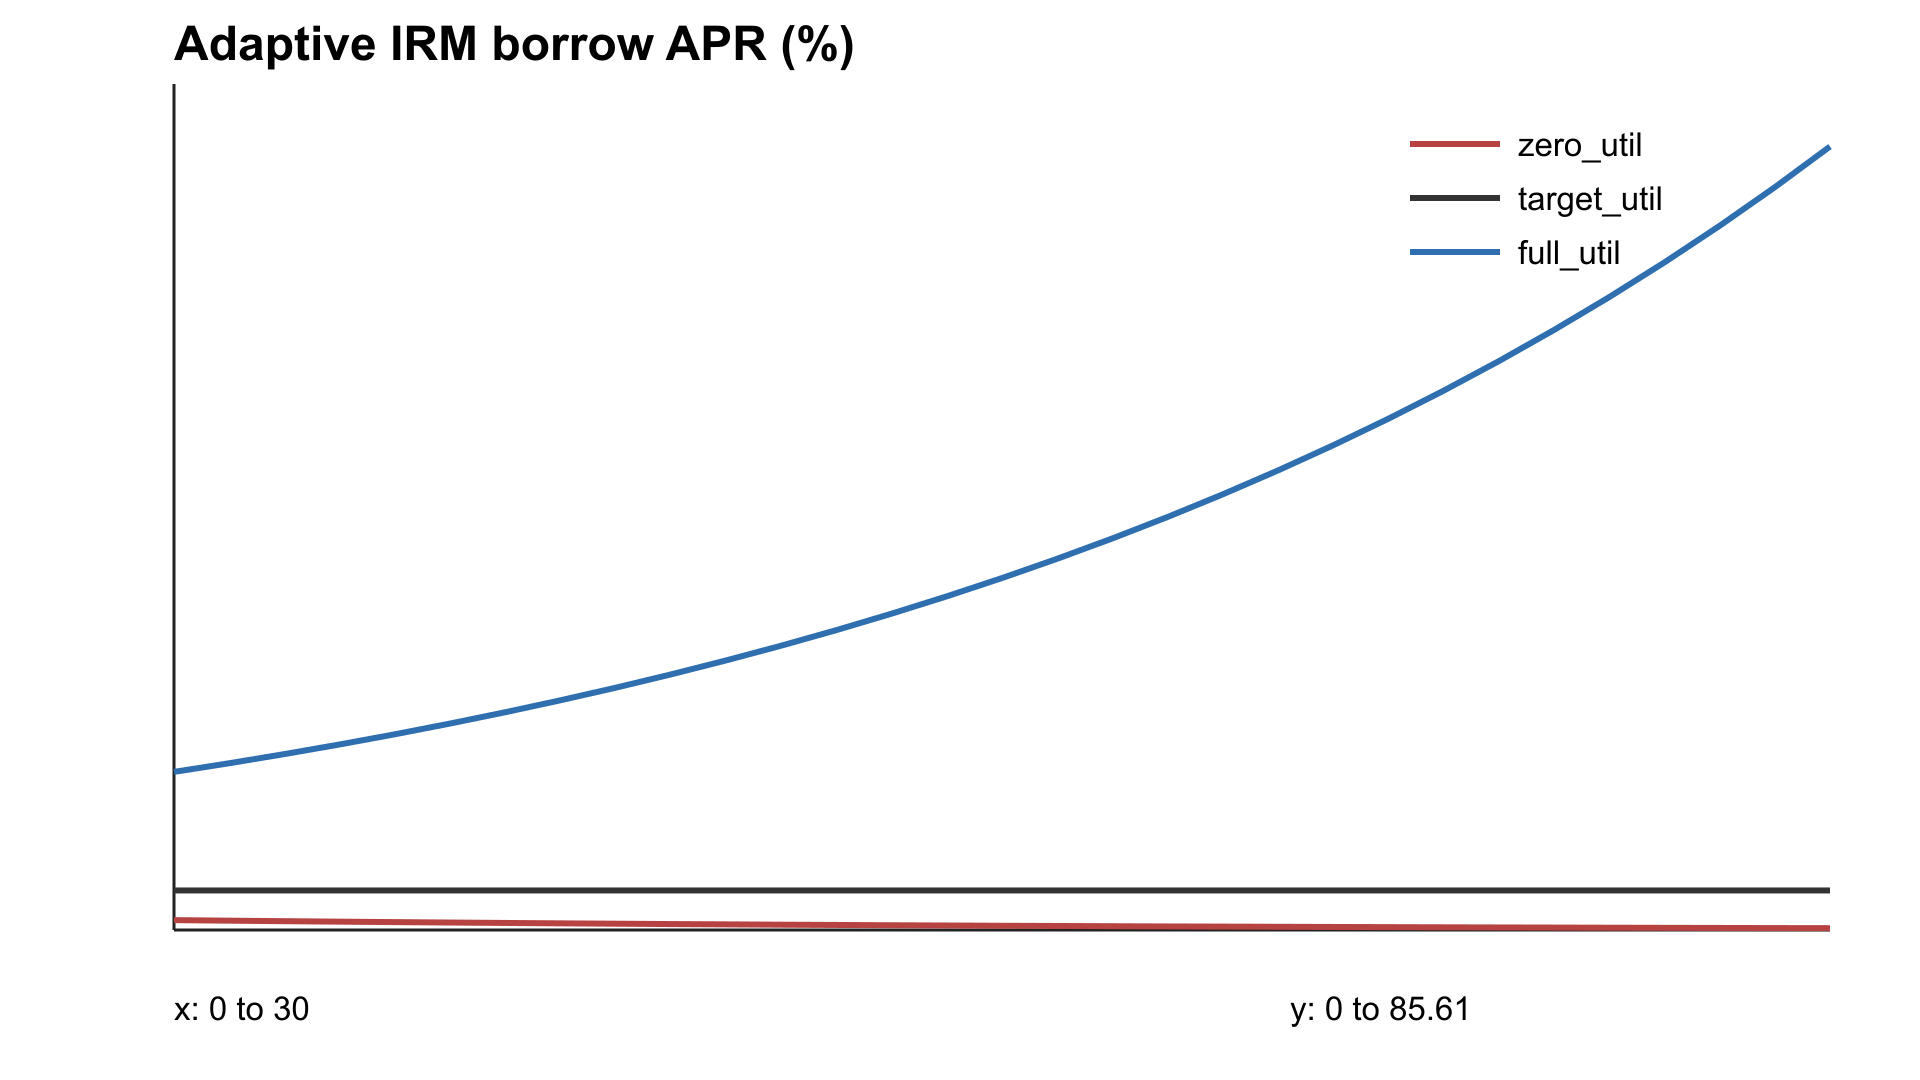
\includegraphics[width=0.78\linewidth]{simulations/figures/adaptive_irm.png}
\caption{Adaptive interest-rate paths under zero, target, and full utilization.}
\end{figure}

\subsection{Live Depth and Slippage}

The second simulation compares constant-product slippage for the same trade size under different live-depth scales. For a trade equal to 5\% of the initial base reserve, slippage is about 476 bps at $1x$ depth, 244 bps at $2x$ depth, and 123 bps at $4x$ depth. This illustrates why balanced hLP live depth matters: preserving spot does not mean preserving the exact curve.

\begin{figure}[t]
\centering
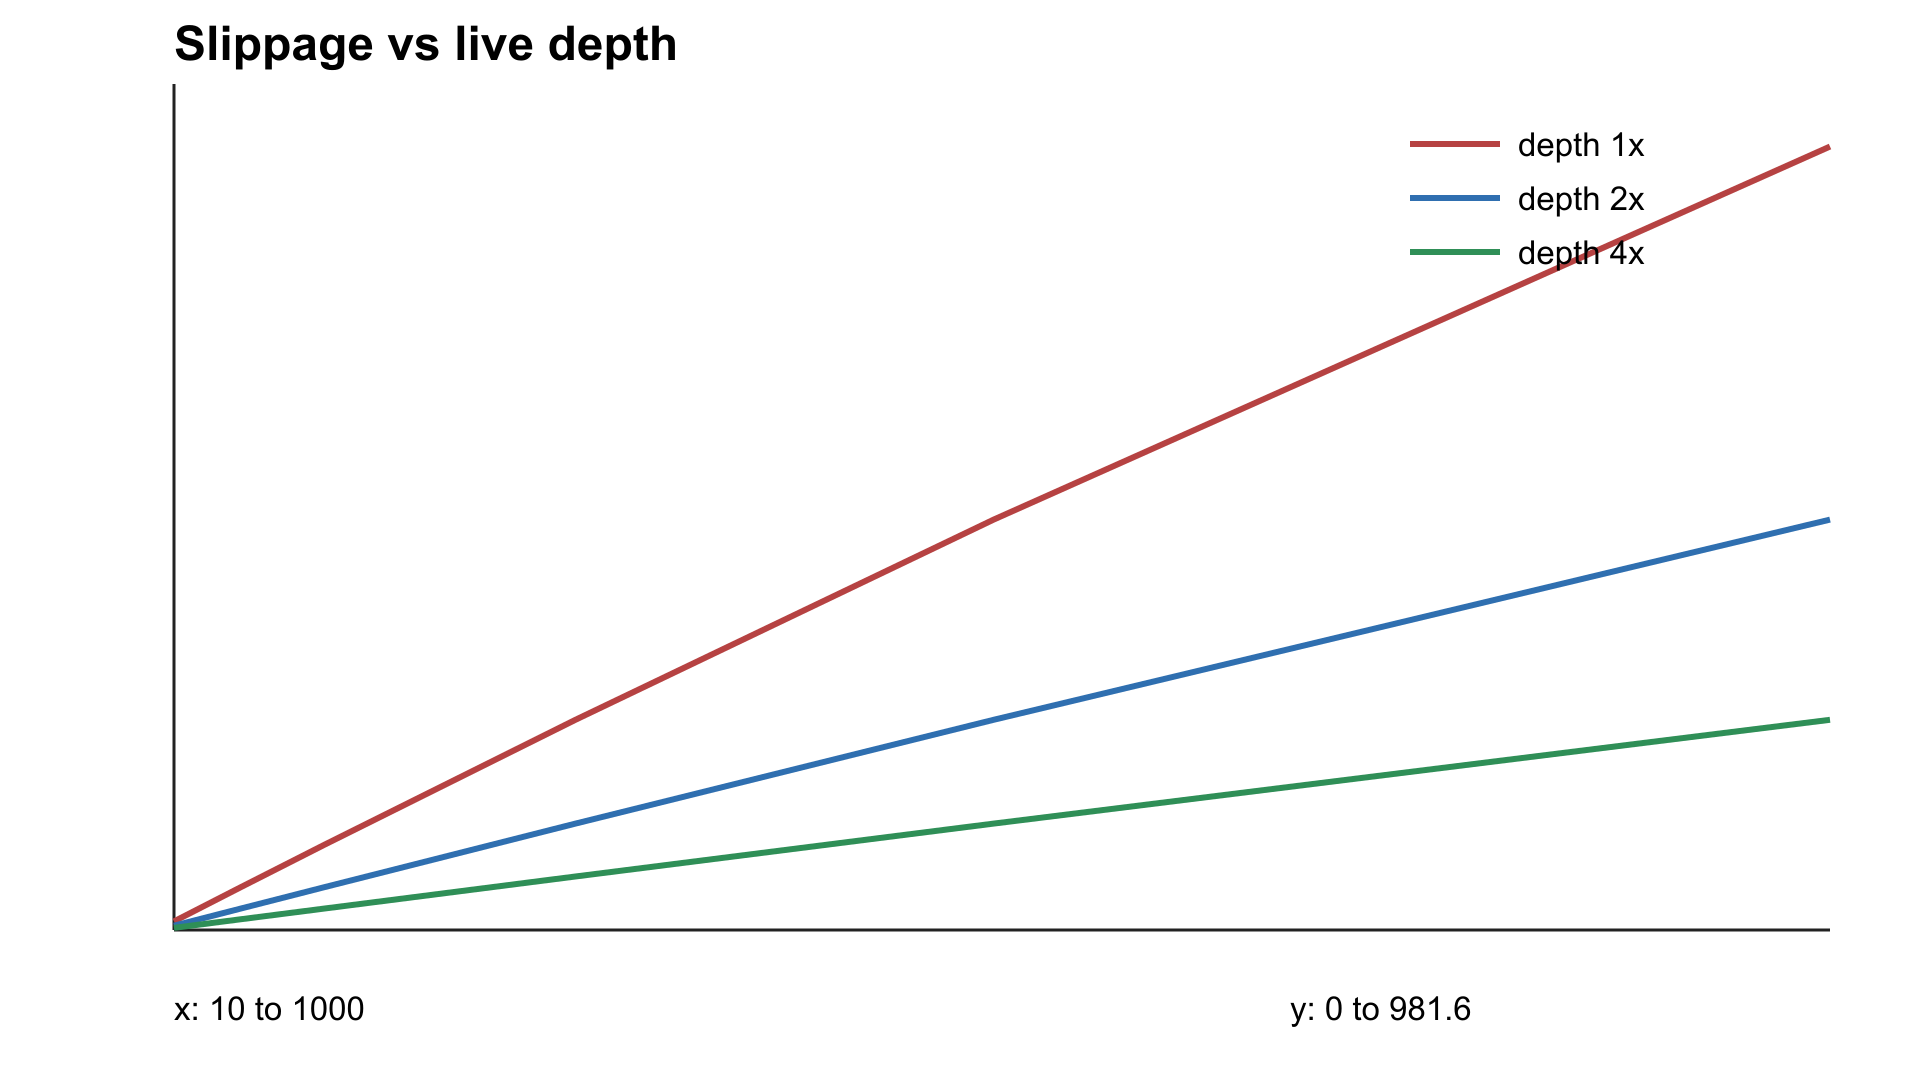
\includegraphics[width=0.78\linewidth]{simulations/figures/slippage_depth.png}
\caption{Slippage under increasing live-depth coordinates for fixed trade sizes.}
\end{figure}

\subsection{hLP Tracking Loss}

The third simulation evaluates \eqref{eq:tracking}. With $E_0=100$, a $+25\%$ price move gives tracking loss about 1.39, a $+50\%$ move gives about 5.05, and a $+100\%$ move gives about 17.16. The convexity is second-order near zero but material for large jumps. Dusk's pre-solve threshold and bounded bisection are designed for exactly this shape: avoid unnecessary computation for small moves, but correct large moves before loss becomes structural.

\begin{figure}[t]
\centering
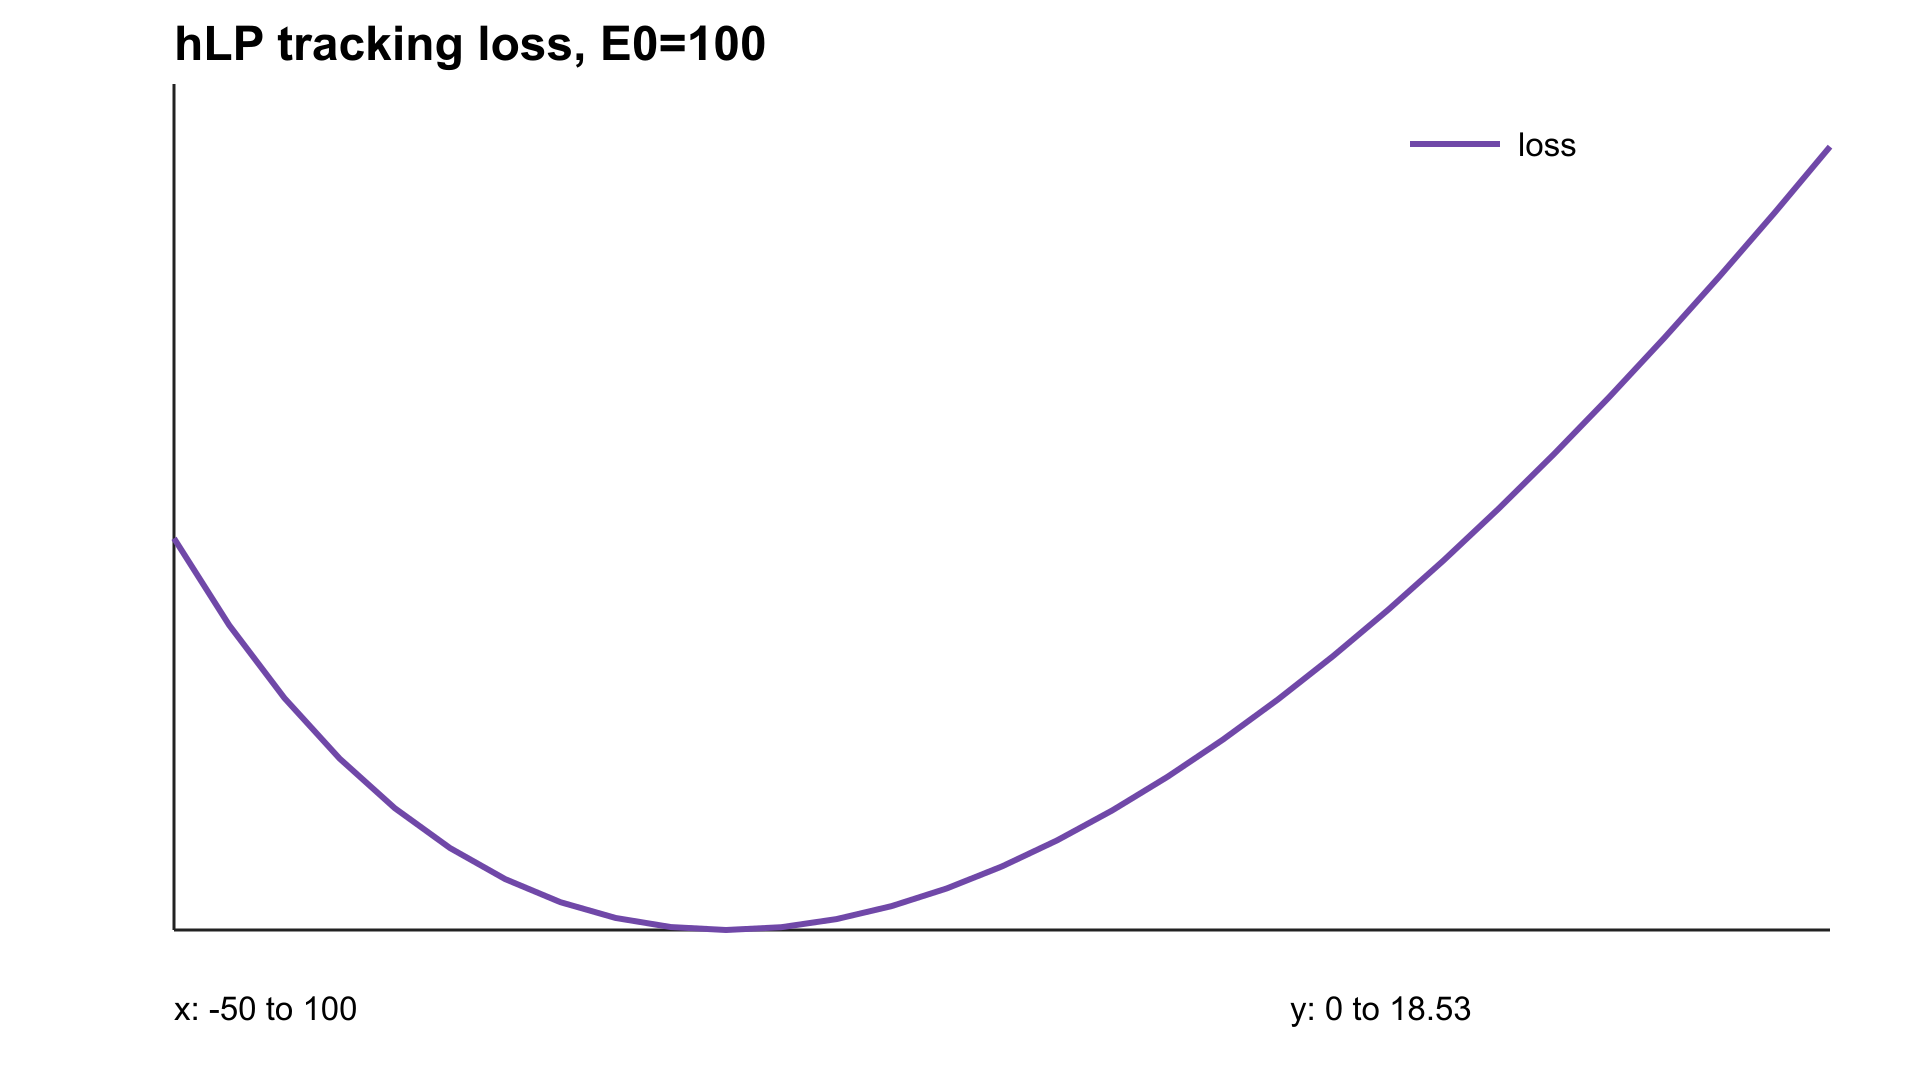
\includegraphics[width=0.78\linewidth]{simulations/figures/hlp_tracking_loss.png}
\caption{Discrete hLP tracking loss for $E_0=100$.}
\end{figure}

\section{Limitations and Future Work}

Dusk does not remove market risk. It changes where risk is measured and settled. The most important limitations are:
\begin{enumerate}
  \item \textbf{Cash constraints.} Live depth can quote, but cash settles. A market with synthetic depth and little cash can still block withdrawals or settlement.
  \item \textbf{Volatility.} hLP rebalancing is more demanding for volatile assets. The mechanism is local, but it is not free.
  \item \textbf{Liquidity quality.} An oracle-less market is only as useful as its own liquidity. Thin or manipulated pools should have strict limits.
  \item \textbf{Parameter risk.} EMA half-lives, divergence thresholds, daily limits, and interest bounds are protocol choices. Bad choices can make a sound invariant unsafe.
  \item \textbf{Implementation risk.} The accounting model is only valuable if the program preserves it across every instruction and every rounding edge.
\end{enumerate}

Future work should include richer simulation against historical flow, formal invariant tests for hLP settlement, explicit stress tests for insurance/socialization, and a clearer empirical framework for deciding which long-tail markets deserve which limits. Dusk's core claim is not that long-tail leverage should be unconstrained. It is that constraints should come from market-local reserves, debt, and liquidity history rather than from external oracle availability alone.

\appendix

\section{Appendix A: Notation}

\begin{center}
\begin{tabular}{ll}
\toprule
Symbol & Definition \\
\midrule
$R_{\cash,i}$ & withdrawable cash reserve for side $i$ \\
$R_{\live,i}$ & live reserve coordinate used for spot and swap math \\
$D_{\cash\text{-}\debt,i}$ & debt that offsets prior cash withdrawals from reserves \\
$R_{\hlp,i}$ & hLP-owned live reserve component \\
$D_{\hlp,i}$ & hLP funding debt \\
$D_{\mathrm{isolated},i}$ & isolated leverage debt \\
$S_{\ylp}$ & normal LP supply \\
$S_{\hlp,t}$ & hLP supply for target side $t$ \\
$I_i$ & borrow index for side $i$ \\
$G_i$ & yield growth index for side $i$ \\
$u_i$ & utilization of side $i$ \\
$r_T$ & adaptive interest-rate anchor at target utilization \\
\bottomrule
\end{tabular}
\end{center}

\section{Appendix B: Constant-Product Identities}

For reserves $(x,y)$ and input $\Delta x$, constant product requires
\begin{equation}
(x+\Delta x)(y-\Delta y)=xy.
\end{equation}
Solving for $\Delta y$ gives
\begin{equation}
\Delta y=\frac{\Delta x\,y}{x+\Delta x}.
\end{equation}
Solving for required input to receive $\Delta y$ gives
\begin{equation}
\Delta x=\frac{\Delta y\,x}{y-\Delta y}.
\end{equation}
Dusk rounds these formulas conservatively in implementation. Outputs round down; required inputs round up.

If both reserves are scaled by $m>1$ and trade size is held fixed, output becomes
\begin{equation}
\Delta y_m=\frac{\Delta x\,my}{mx+\Delta x}.
\end{equation}
The execution price approaches spot as $m$ grows. This is the formal reason balanced hLP live depth can improve finite-trade execution while preserving spot.

\section{Appendix C: hLP Tracking Derivation}

For a constant-product LP, inventory value is approximately geometric in price. With price ratio $r$, LP value scales as $\sqrt r$ in units of the original portfolio benchmark. A 2x leveraged LP seeks to square that exposure. In the continuous limit, this tracks $r$ rather than $\sqrt r$.

With discrete rebalancing, a price move occurs before the vault can perfectly reset its leverage. The local tracking gap is
\begin{equation}
L_{\mathrm{track}}=E_0(\sqrt r-1)^2.
\end{equation}
The pre-adjustment that cancels the gap in the exogenous-ratio case is
\begin{equation}
\Delta_{\mathrm{pre}}=E_0(\sqrt r-1),
\end{equation}
with sign determined by whether $r>1$ or $r<1$. Dusk uses this as an initial guess, then solves against the simulated post-adjustment ratio because the adjustment changes reserves.

\section{Appendix D: Simulation Reproducibility}

The deterministic simulation script writes three CSV files:
\begin{itemize}
  \item \texttt{adaptive\_irm.csv};
  \item \texttt{slippage\_depth.csv};
  \item \texttt{hlp\_tracking\_loss.csv}.
\end{itemize}
It also writes SVG previews and PNG renderings used by this document. The script intentionally avoids external APIs. The Raydium notebook statistics used in the introduction are cited as motivation only and are not regenerated by the paper.

\section{Appendix E: Implementation Mapping}

The paper's notation maps to Dusk program concepts as follows:
\begin{center}
\begin{tabular}{lll}
\toprule
Paper object & Program-level concept & Reason for separation \\
\midrule
$R_{\cash}$ & reserve vault cash & settles transfers \\
$R_{\live}$ & live reserve field & prices swaps \\
$D_{\cash\text{-}\debt}$ & fixed debt shares/index & preserves borrow neutrality \\
$R_{\hlp}$ & hLP live reserve fields & names synthetic depth \\
$D_{\hlp}$ & hLP debt shares/principal & prices hLP funding \\
$D_{\mathrm{isolated}}$ & leverage debt buckets & isolates spot-margin positions \\
$G_i$ & fee/interest growth indexes & distributes yield outside principal \\
\bottomrule
\end{tabular}
\end{center}

The implementation should be reviewed by transition class. Each instruction should answer three questions:
\begin{enumerate}
  \item Which live reserve coordinate can it change?
  \item Which cash balance can it spend or credit?
  \item Which debt, share, or yield liability changes with it?
\end{enumerate}
If those answers are inconsistent, the invariant is likely broken.

\section{Appendix F: Normal Borrow Lifecycle}

A normal borrow position is not an isolated leverage position and not an hLP vault. It is a fixed-debt position tied to recognized collateral on the opposite side of the market. The lifecycle is:
\begin{enumerate}
  \item the user deposits collateral on side $c$;
  \item the market recognizes a debt-bearing portion of that collateral for debt side $d$;
  \item the user borrows side $d$;
  \item interest accrues through side $d$'s borrow index;
  \item the user repays or becomes liquidatable if recognized collateral value falls below debt requirements.
\end{enumerate}

The key accounting step is the borrow. If a user borrows amount $a$ of side $d$, cash decreases by $a$ and cash-backed debt increases by $a$. The live reserve coordinate is unchanged. This is why a borrow does not look like a swap. A swap changes the market price because it trades one side of inventory for another. A borrow changes the composition of one side between cash and debt claim.

Collateral recognition is deliberately stricter than wallet balance. Suppose a user has total collateral $C_c$ and debt $D_d$. Dusk computes a recognized collateral amount
\begin{equation}
C_c^{\mathrm{rec}}=\min(C_c,C_c^{\mathrm{cap}}(D_d)),
\end{equation}
where the cap depends on debt value and market configuration. This prevents a user from depositing a large idle balance and then relying on that entire balance as if it were actively protecting each debt bucket. In a two-sided market, collateral recognition must know which side is backing which debt.

Repayment has a non-compounding interest split. If total debt is $D$, principal is $P$, and a user repays $r$, Dusk splits the repayment into
\begin{equation}
p=r\frac{P}{D},\qquad \iota=r-p,
\end{equation}
with conservative rounding. The principal portion returns to the reserve cash coordinate. The interest portion is a yield liability and is routed to the interest vault. The important invariant is not "cash increases by repayment." It is "principal cash and yield liabilities increase in the correct proportions while live debt falls."

This lifecycle is intentionally pair-local. No global account says that a user is healthy across all markets. A position is healthy because this market's conservative value of recognized collateral exceeds this market's effective debt. That isolation is what lets a risky long-tail pair fail locally.

\section{Appendix G: hLP Lifecycle and Settlement}

hLP has a different lifecycle from normal borrowing. It is a vault-level leveraged LP strategy rather than a user-specific debt position. For target asset $t$:
\begin{enumerate}
  \item user deposits target asset $t$;
  \item the vault funds the opposite leg $o$;
  \item the market mints yLP exposure to the hLP vault;
  \item the vault records funding debt shares in $o$;
  \item the user receives hLP shares in target-side vault equity.
\end{enumerate}

The opening transaction adds target cash and funded live depth. If target is base, the base cash reserve increases from the deposit, while quote hLP live reserve increases from the funded leg. The funded leg is not the same as a normal borrower withdrawing quote cash. It is a live-depth coordinate tied to vault accounting and funding debt. This is why the invariant has a named $R_{\hlp}$ term.

Settlement reverses the aggregate exposure proportionally. A user burning fraction $\phi$ of hLP supply removes approximately $\phi$ of the vault's yLP shares, $\phi$ of its hLP live depth, and $\phi$ of its funding debt shares. The actual target amount returned depends on the reserves, debt repayment, interest, cash headroom, and settlement references. The proportional rule prevents a withdrawing hLP holder from selecting only favorable pieces of the aggregate vault.

The hLP settlement problem is harder than a normal LP withdrawal because three prices matter:
\begin{enumerate}
  \item the current spot price, which determines the live AMM coordinate;
  \item the cached settlement price, which limits stale or manipulated settlement;
  \item the effective price after unwinding debt and yLP exposure.
\end{enumerate}
If these diverge too much, a mathematically positive NAV can still be unsafe to settle. Dusk treats this as a reason to block or constrain settlement rather than a reason to pretend the vault is insolvent.

Pending rebalance is a liveness device. If a desired hLP lever-up is cash-constrained, Dusk can carry the unexecuted portion as pending rebalance instead of blocking all swaps. This keeps the market usable while preserving the fact that the hLP vault has not reached its target state. The pending value is debt and depth intent, not a hidden cash claim.

\section{Appendix H: Isolated Leverage Lifecycle}

Isolated spot-margin leverage is a user-level position. It is useful to describe it separately because it shares the same swap curve and interest model but not the same health accounting as normal borrower positions.

Opening a long target-side position follows this pattern:
\[
\begin{aligned}
&\text{margin in debt asset}
\rightarrow \text{internal borrow of debt asset}\\
&\rightarrow \text{GAMM swap into collateral asset}
\rightarrow \text{isolated collateral vault}.
\end{aligned}
\]
The user pays price impact immediately. If the market is thin, the position opens with less collateral and lower closeout value. This avoids a common lending-market illusion: leverage cannot be opened at a linear oracle mark and then liquidated through a nonlinear AMM without creating a gap.

Increasing leverage adds more isolated debt and swaps the new notional into collateral. Decreasing leverage sells some collateral back through the GAMM and repays debt. Closing sells all collateral, repays debt, routes realized interest, and returns residual to the owner. Liquidation sells collateral when closeout value no longer satisfies maintenance conditions. If the swap output is less than debt, the position's remaining debt shares can be written off and reflected in the market's live reserve state.

The isolated debt bucket contributes to utilization:
\begin{equation}
u_i=\frac{D_{\cash\text{-}\debt,i}+D_{\hlp,i}+D_{\mathrm{isolated},i}}
{D_{\cash\text{-}\debt,i}+D_{\hlp,i}+D_{\mathrm{isolated},i}+R_{\cash,i}}.
\end{equation}
But isolated leverage debt does not become normal margin debt. This matters because normal borrower health is based on recognized debt-bearing collateral, while isolated leverage health is based on closeout value of a specific collateral vault. Mixing the two would allow a user-level leveraged trade to pollute market-level borrower health checks.

The leverage system therefore has a clean rule: all price exposure is executed through the GAMM, all debt pays the side-specific interest rate, but position health is checked in the position's own accounting domain.

\section{Appendix I: Risk Controls as Time Filters}

Dusk's risk controls can be understood as time filters over three quantities:
\begin{enumerate}
  \item price, through symmetric and directional EMAs;
  \item depth, through side-specific liquidity EMAs;
  \item invariant scale, through $K$ and liquidity EMAs.
\end{enumerate}

The directional EMA is designed to be conservative for collateral. If spot moves in a direction that makes collateral look better, the directional reference can lag. If spot moves in a direction that makes collateral worse, the reference can follow more quickly. The exact implementation is simple, but the economic intent is important: users should not be able to borrow against a transient favorable mark as easily as they can be liquidated against an adverse mark.

The liquidity EMA limits the effect of sudden depth changes. A market can be deepened in one transaction, but risk does not have to recognize the entire new depth immediately. This is important for oracle-less markets because depth itself is part of the defense against manipulation. If risk recognized all depth instantly, an attacker could temporarily deepen a pool, borrow against it, then remove or reverse the depth.

The $K$ drawdown guard watches the aggregate invariant scale. A large fall in $K$ relative to its EMA is a warning that the market's liquidity state changed too abruptly. It does not identify every possible bad state, but it gives the protocol a simple circuit breaker that is native to the AMM.

Daily borrow limits are also depth-derived. A side's borrow limit can be computed as a fraction of its liquidity EMA rather than a fixed token amount. This makes limits scale with observed market depth and avoids hardcoding per-asset borrow ceilings before the market has history.

\section{Appendix J: Failure Modes}

The invariant clarifies several failure modes that reviewers should test.

\textbf{Cash-live confusion.} A transition credits live reserve without crediting cash or a named synthetic coordinate. This creates quote depth without a liability owner. The review question is: if this live reserve is later withdrawn, which cash or debt path pays for it?

\textbf{Debt-domain confusion.} A transition treats hLP funding debt as cash-backed borrower debt, or treats isolated leverage debt as normal borrower debt. This can distort utilization, health, and liquidation. Each debt bucket should have a clear health domain.

\textbf{Yield-principal confusion.} Fees or interest are added to principal reserves without corresponding share/yield accounting. This can dilute or overpay LPs depending on when shares are minted and burned. Dusk avoids this by routing realized yield through growth indexes.

\textbf{Rounding drift.} Conservative rounding is necessary, but repeated rounding can create small residuals. The implementation should assert share backing and fee backing after transitions that touch reserves or liabilities.

\textbf{Settlement optimism.} A vault has positive mark-to-market NAV but insufficient cash to settle. This is not a contradiction. The correct behavior is to enforce cash and divergence guards rather than allowing synthetic live depth to become a cash withdrawal.

\textbf{Same-transaction manipulation.} A user moves spot, borrows against the moved spot, and reverses the trade. Cached EMA references, directional price, and liquidity caps exist to make this uneconomic or invalid.

\section{Appendix K: Deterministic Simulation Tables}

The adaptive IRM simulation uses the current paper constants: target utilization $90\%$, steepness $4$, initial target APR $4\%$, minimum target APR $0.1\%$, maximum target APR $200\%$, and adjustment speed $20$ per year.

\begin{center}
\begin{tabular}{lccc}
\toprule
Scenario & Utilization & Day 0 borrow APR & Day 30 borrow APR \\
\midrule
Idle & $0\%$ & $1.0000\%$ & $0.1844\%$ \\
Target & $90\%$ & $4.0000\%$ & $4.0000\%$ \\
Full & $100\%$ & $16.0000\%$ & $79.2786\%$ \\
\bottomrule
\end{tabular}
\end{center}

The live-depth simulation holds trade size fixed relative to the initial reserve and scales both reserves. For a 5\% trade:
\begin{center}
\begin{tabular}{lccc}
\toprule
Depth scale & $1x$ & $2x$ & $4x$ \\
\midrule
Slippage & $476.19$ bps & $243.90$ bps & $123.46$ bps \\
\bottomrule
\end{tabular}
\end{center}

The hLP tracking-loss simulation sets $E_0=100$:
\begin{center}
\begin{tabular}{lccccc}
\toprule
Price move & $-50\%$ & $-25\%$ & $+25\%$ & $+50\%$ & $+100\%$ \\
\midrule
Tracking loss & $8.58$ & $1.79$ & $1.39$ & $5.05$ & $17.16$ \\
Pre-adjustment & $29.29$ & $13.40$ & $11.80$ & $22.47$ & $41.42$ \\
\bottomrule
\end{tabular}
\end{center}

These numbers are deliberately simple. Their purpose is not prediction; it is to make the qualitative claims falsifiable. If a future implementation changes constants or rounding, these tables should change in a predictable way.

\section{Appendix L: Review Checklist}

For an implementation audit, the following questions are higher value than checking whether a function name matches the paper:
\begin{enumerate}
  \item Does every instruction preserve \eqref{eq:gamm} for both sides?
  \item Can a transition increase live reserve without increasing cash, debt, or hLP live depth?
  \item Can hLP funding debt be used as if it were same-side cash-backed debt?
  \item Can isolated leverage debt enter normal borrower health?
  \item Can yield be claimed twice through stale checkpoints?
  \item Can a fee or interest liability exceed its vault backing?
  \item Can a user withdraw cash backed only by synthetic live depth?
  \item Can a same-transaction spot move increase borrow capacity without EMA recognition?
  \item Can liquidation socialization exceed the caller's declared maximum?
  \item Can a config update make existing debt immediately unsafe without timelock or circuit breaker semantics?
\end{enumerate}

The desired answer to the first question is mathematical. The desired answer to the remaining questions is a combination of account constraints, state assertions, and tests. Dusk is a compact mechanism only if these checks remain local.

\section{Appendix M: Comparison Notes}

This appendix gives a more explicit comparison matrix. It is not meant to rank protocols. It is meant to explain which parts of Dusk are borrowed from a broader AMM tradition and which parts are specific to Dusk's accounting model.

\begin{center}
\begin{tabular}{p{0.18\linewidth}p{0.23\linewidth}p{0.23\linewidth}p{0.23\linewidth}}
\toprule
System & Primary object & Price/risk reference & Relevant lesson for Dusk \\
\midrule
StableSwap & near-parity liquidity invariant & pool reserves & invariant shape can encode expected asset behavior \\
CryptoPools & dynamic-peg AMM & internal price adaptation & AMMs can manage price references internally \\
Morpho IRM & lending market rate controller & utilization error & rate level can adapt rather than be hardcoded \\
Yield Basis & leveraged Curve LP exposure & Curve pool, crvUSD, LEVAMM & 2x LP can hedge geometric LP value \\
Likwid & AMM-integrated lending framework & protocol-specific AMM state & insurance and lending can be closer to liquidity \\
Dusk & pair-local GAMM state & live reserves plus cached risk books & swaps, lending, hLP, and liquidation share one reserve model \\
\bottomrule
\end{tabular}
\end{center}

The Yield Basis comparison deserves special care because it is tempting to oversimplify it. Yield Basis does not merely "externally rebalance." It defines a leveraged AMM around Curve LP tokens and a VirtualPool path that makes arbitrage practical. Its economic model depends on crvUSD debt, Curve LP oracles, and fee routing that supports rebalancing. This is a coherent design. Dusk's claim is narrower: when the AMM, debt book, and leveraged LP vault are the same market, the protocol can update hLP state in the same instruction family that changes reserves.

The Morpho comparison is also specific. Dusk does not copy Morpho's market architecture. It borrows the useful idea that the right borrow-rate level is market-discovered. A target utilization is a policy choice, but the long-run level of $r_T$ should adapt to persistent demand. That matters more in long-tail markets because governance cannot manually tune every pair.

The Curve comparison is philosophical as much as mathematical. Curve's work showed that an AMM can embed assumptions about the traded assets into the invariant and price dynamics. Dusk embeds a different assumption: in a pair-local credit market, the reserve coordinate should also be the liquidation coordinate. This is why impact-aware collateral valuation is not an add-on; it is the lending analogue of AMM slippage.

\section{Appendix N: Parameter Families}

Dusk has several parameter families. They should not be treated as independent knobs.

\textbf{Fee parameters.} Swap fee, manager fee, and protocol fee determine how much trading flow becomes yield or revenue. Higher fees can improve LP yield but worsen execution, liquidation recovery, and leverage closeout. In a GAMM, fee choice affects both traders and borrowers because liquidation and leverage paths use the same curve.

\textbf{Interest parameters.} Target utilization, curve steepness, anchor speed, min APR, max APR, and max per-step adjustment define the borrow-rate controller. Increasing steepness gives faster immediate response to utilization. Increasing adaptation speed lets the anchor chase demand faster. Both can protect cash but can also make borrower costs more volatile.

\textbf{Risk reference parameters.} EMA half-lives, directional half-lives, spot-EMA divergence bounds, and $K$ drawdown bounds determine how quickly risk books accept new market state. Short half-lives make the system responsive but easier to manipulate. Long half-lives make the system conservative but slower to list or scale new liquidity.

\textbf{Borrow limits.} Daily borrow limits and recognized-collateral caps determine how much debt can be opened relative to observed liquidity. These parameters are especially important for long-tail markets. A pair may have enough spot volume to justify listing but not enough historical depth to justify high leverage.

\textbf{hLP parameters.} Target leverage, pre-solve threshold, bisection iteration budget, settlement divergence, and emergency exit haircut govern the hLP vaults. These parameters decide when the protocol spends compute to improve tracking, when it carries pending rebalance, and when it refuses settlement.

\textbf{Liquidation parameters.} Close factor, liquidation incentive, insurance funding, maximum incentive, and socialization caps determine how losses move. These should be calibrated against actual recovery depth. If incentives are too low, liquidations may not run. If incentives are too high, borrowers lose more collateral than necessary and insurance may be starved.

The important point is compositional. A higher hLP target depth changes slippage, which changes leverage closeout, which changes liquidation recovery, which changes safe borrow caps. Parameter review should therefore be scenario-based rather than one-number-at-a-time.

\section{Appendix O: Threat Model and Non-goals}

Dusk's threat model includes manipulation of spot price, temporary manipulation of live depth, stale risk references, cash exhaustion, bad debt after liquidation, malicious or mistaken configuration updates, and arithmetic/rounding edge cases. The protocol responds with cached references, impact-aware valuation, cash checks, insurance, socialization caps, timelocks, and invariant assertions.

The design does not attempt to protect against every offchain market event. If an asset's fundamental price collapses and the market has no buyers, a pair-local system will still produce losses. Dusk's claim is not that local accounting creates external liquidity. It is that the local market should not overstate recoverable value in the first place.

Dusk also does not attempt to be a universal cross-margin system. Cross-margin is useful for capital efficiency, but it spreads failure domains. Dusk chooses isolation: a market's debt is backed by that market's recognized collateral and settled through that market's reserves. This is a deliberate tradeoff against global netting.

The design does not assume that hLP always improves safety. hLP can improve depth and create useful one-sided LP exposure, but it adds funding debt and settlement complexity. The right hLP size for a market may be zero. The mechanism exists so that when hLP is useful, it is accounted for explicitly.

Finally, Dusk does not remove governance risk. Parameter changes, manager authority, and emergency controls are part of the system. A research paper can define the invariant, but deployment safety also depends on operational procedures, monitoring, and conservative rollout.

\section{Appendix P: Empirical Evaluation Plan}

The deterministic simulations in this draft are sanity checks. A production research program should add empirical evaluation in four layers.

\textbf{Historical replay.} Replay external price and volume data for representative Solana pairs. The replay should compare no-hLP, hLP without pre-solve, and hLP with pre/post solve. Outputs should include LP return, tracking loss, funding cost, liquidations, and cash exhaustion events.

\textbf{Adversarial flow.} Construct worst-case sequences: spot pump before borrow, depth add before borrow, depth remove after borrow, repeated small swaps to manipulate EMA, sudden $K$ drawdown, and hLP withdrawal under cash stress. These flows should be run against exact program math, not only paper formulas.

\textbf{Parameter sweeps.} Sweep EMA half-lives, divergence thresholds, target utilization, rate speed, hLP loss thresholds, and borrow caps. The goal is not to find one universal setting. It is to understand which parameters dominate failure probability for different market classes.

\textbf{Operational metrics.} Track live reserve, cash reserve, debt by bucket, hLP NAV, pending rebalance, utilization, risk EMAs, insurance available, and socialized loss. A monitoring dashboard should expose these quantities directly. If operators only watch price and TVL, they will miss the state variables that make Dusk different.

The empirical standard should be falsifiable: a market class is supported only if its historical and adversarial simulations stay within predefined loss, cash, and liquidation bounds. This is the practical meaning of "long-tail support" in Dusk. The protocol can list markets that oracle systems cannot, but each market should earn that permission through its own depth history and stress behavior.

\section{Appendix Q: State-Transition Equations}

This appendix records the idealized state transitions in one place. The implementation has rounding, account validation, fees, and event emission; the equations below are the clean accounting model.

\textbf{Swap.} For input side $x$, output side $y$, input amount after fee $\Delta x$, and output $\Delta y$:
\begin{align}
\Delta y &= \frac{\Delta x R_{\live,y}}{R_{\live,x}+\Delta x},\\
R_{\live,x}' &= R_{\live,x}+\Delta x,\\
R_{\cash,x}' &= R_{\cash,x}+\Delta x,\\
R_{\live,y}' &= R_{\live,y}-\Delta y,\\
R_{\cash,y}' &= R_{\cash,y}-\Delta y.
\end{align}
The fee portion is not included in $\Delta x$; it is routed to fee accounting. If hLP pre/post checkpoints run around the swap, they are additional balanced live-depth transitions.

\textbf{Borrow.} For debt side $d$ and borrow amount $a$:
\begin{align}
R_{\cash,d}' &= R_{\cash,d}-a,\\
D_{\cash\text{-}\debt,d}' &= D_{\cash\text{-}\debt,d}+a,\\
R_{\live,d}' &= R_{\live,d}.
\end{align}
The borrow is allowed only if collateral recognition, market health, daily limit, and cash headroom checks pass.

\textbf{Repay.} For repayment $r$, total debt $D$, and principal $P$:
\begin{align}
p &= rP/D,\\
\iota &= r-p,\\
R_{\cash,d}' &= R_{\cash,d}+p,\\
D_{\cash\text{-}\debt,d}' &= D_{\cash\text{-}\debt,d}-r,\\
\mathrm{InterestVault}_d' &= \mathrm{InterestVault}_d+\iota.
\end{align}
The exact program uses conservative rounding so interest is not underfunded.

\textbf{Add yLP.} For a two-sided deposit $(a_\base,a_\qasset)$:
\begin{align}
\Delta S_{\ylp} &=
\min\left(
S_{\ylp}\frac{a_\base}{R_{\live,\base}},
S_{\ylp}\frac{a_\qasset}{R_{\live,\qasset}}
\right),\\
R_{\cash,i}' &= R_{\cash,i}+a_i,\\
R_{\live,i}' &= R_{\live,i}+a_i.
\end{align}
At first deposit, supply is proportional to $\sqrt{a_\base a_\qasset}$ less permanently locked minimum liquidity.

\textbf{Remove yLP.} For burn amount $s$:
\begin{align}
a_i &= s\frac{R_{\live,i}}{S_{\ylp}},\\
R_{\cash,i}' &= R_{\cash,i}-a_i,\\
R_{\live,i}' &= R_{\live,i}-a_i,\\
S_{\ylp}' &= S_{\ylp}-s.
\end{align}
The withdrawal is constrained by cash reserves. A live reserve claim that cannot be paid in cash cannot leave the vault.

\textbf{Open hLP.} For target asset $t$, opposite asset $o$, target deposit $a_t$, and funded amount $a_o$:
\begin{align}
R_{\cash,t}' &= R_{\cash,t}+a_t,\\
R_{\live,t}' &= R_{\live,t}+a_t,\\
R_{\hlp,o}' &= R_{\hlp,o}+a_o,\\
R_{\live,o}' &= R_{\live,o}+a_o,\\
D_{\hlp,o}' &= D_{\hlp,o}+a_o.
\end{align}
The vault receives yLP and the user receives hLP shares against NAV delta.

\textbf{Close hLP.} For burn fraction $\phi=s/S_{\hlp,t}$:
\begin{align}
\Delta \mathrm{yLP}_{\hlp} &= \phi\,\mathrm{yLP}_{\hlp},\\
\Delta D_{\hlp,o} &= \phi\,D_{\hlp,o},\\
\Delta R_{\hlp,i} &= \phi\,R_{\hlp,i}.
\end{align}
The realized target output depends on withdrawing yLP, repaying funding debt, routing interest, and cash constraints.

\textbf{Open isolated leverage.} For margin $m$, multiplier $L$, debt side $d$, and collateral side $c$:
\begin{align}
d &= m(L-1),\\
n &= m+d,\\
c_{\mathrm{out}} &= \frac{n_{\mathrm{after\ fee}}R_{\live,c}}{R_{\live,d}+n_{\mathrm{after\ fee}}}.
\end{align}
The debt side cash reserve decreases by borrowed amount $d$, and the notional swap updates the live AMM reserves. The position stores debt shares and collateral amount.

\textbf{Close isolated leverage.} For collateral $c$ and debt $D$:
\begin{align}
v &= \frac{c_{\mathrm{after\ fee}}R_{\live,d}}{R_{\live,c}+c_{\mathrm{after\ fee}}},\\
\mathrm{residual} &= \max(v-D,0),\\
\mathrm{shortfall} &= \max(D-v,0).
\end{align}
If shortfall exists during liquidation, the position can write off remaining isolated debt shares and reduce live reserve accordingly.

\section{Appendix R: Deployment and Monitoring Notes}

A Dusk deployment should expose the same accounting split that this paper uses. The minimum useful dashboard is not price and TVL; it is:
\begin{itemize}
  \item cash reserve by side;
  \item live reserve by side;
  \item cash-backed debt by side;
  \item hLP live reserve by side;
  \item hLP funding debt and NAV by target vault;
  \item isolated leverage debt by side;
  \item utilization and rate-at-target by side;
  \item spot price, price EMA, directional price EMA, and divergence;
  \item liquidity EMA and $K$ EMA;
  \item insurance available and cumulative socialized loss.
\end{itemize}

The monitoring rule is simple: if operators cannot explain a change in $R_{\live}$ as a change in cash, cash-backed debt, or hLP live depth, something is wrong. If operators cannot explain a change in utilization as a change in debt bucket or cash reserve, something is wrong. If hLP NAV moves but the underlying yLP, funding debt, or settlement price did not move, something is wrong.

Rollout should be staged by market class. A stable or highly liquid pair can tolerate larger limits and faster recognition. A volatile long-tail pair should start with smaller daily borrow limits, stricter divergence bounds, lower hLP caps, and conservative hLP settlement. The point of Dusk is permissionless market formation, not permissionless leverage at arbitrary size.

Emergency controls should be described operationally before launch. Reduce-only mode, global reduce-only mode, manager changes, and config timelocks are not mere admin functions. They are part of the protocol's response to parameter error, market manipulation, and implementation bugs. A paper can define the normal invariant, but a deployment needs a procedure for what to do when a circuit breaker fires.

Finally, monitoring should treat hLP and isolated leverage as first-class risk sources. Both can improve capital efficiency and market usability. Both can also consume cash headroom and increase liquidation load. A dashboard that aggregates all debt into one number loses the exact information Dusk worked to preserve.

\section{Appendix S: Worked Reserve Example}

This appendix gives a small numerical example. The numbers are deliberately simple and ignore fees, rounding, share minting, and interest accrual. The purpose is to show which state variables move and which do not.

Consider a fresh market with
\[
R_{\cash,\base}=1000,\quad R_{\cash,\qasset}=1000,\quad
D_{\cash\text{-}\debt,\base}=D_{\cash\text{-}\debt,\qasset}=0,\quad
R_{\hlp,\base}=R_{\hlp,\qasset}=0.
\]
Then $R_{\live,\base}=1000$, $R_{\live,\qasset}=1000$, $K=10^6$, and the spot price is one quote token per base token.

\textbf{Normal borrow.} A borrower posts recognized base-side collateral and borrows 100 quote tokens. The quote reserve vault pays 100 tokens out, so quote cash decreases. The quote debt bucket increases by the same amount:
\[
R_{\cash,\qasset}'=900,\qquad
D_{\cash\text{-}\debt,\qasset}'=100,\qquad
R_{\live,\qasset}'=900+100=1000.
\]
No base reserve changes. Therefore spot price and $K$ are unchanged. This is the simplest expression of price-neutral borrowing. The market has less withdrawable quote cash, but the AMM coordinate has not moved.

\textbf{Swap after borrowing.} Now a trader swaps 100 base into the market. With constant-product output,
\[
\Delta \qasset = \frac{100\cdot 1000}{1000+100}=90.9091.
\]
The live base reserve increases to 1100 and the live quote reserve decreases to 909.0909. Cash moves because the trade physically pays base in and quote out:
\[
R_{\cash,\base}'=1100,\qquad
R_{\cash,\qasset}'=809.0909.
\]
The quote debt bucket is still 100, so the invariant continues to explain the live quote reserve:
\[
R_{\live,\qasset}'=809.0909+100+0=909.0909.
\]
The swap changes price; the borrow did not. This distinction is the reason Dusk keeps cash and live reserve separate.

\textbf{Balanced hLP depth.} Return to the initial 1000/1000 market and open an idealized base-target hLP vault that adds 100 base cash and 100 quote hLP live depth. This is the price-neutral balanced case:
\[
R_{\cash,\base}'=1100,\quad
R_{\hlp,\qasset}'=100,\quad
D_{\hlp,\qasset}'=100,
\]
\[
R_{\live,\base}'=1100,\qquad
R_{\live,\qasset}'=1100.
\]
The spot price is still one, while the curve depth has increased. This is not ordinary borrowing. Ordinary quote borrowing would remove quote cash and add quote cash-backed debt, leaving quote live reserve unchanged. hLP funding debt instead supports a vault position whose live reserve contribution is named by $R_{\hlp,\qasset}$.

\textbf{Unbalanced hLP attempt.} If the same vault tried to add 100 base and only 50 quote live depth, the live reserves would become 1100/1050 and the spot price would move. A Dusk implementation can decide whether to solve for balanced amounts, carry pending rebalance, or reject based on divergence and settlement parameters. The paper's invariant does not say every hLP action is price neutral. It says the source of every live reserve change is auditable.

\textbf{Audit table.} The following table summarizes the state transitions.
\begin{center}
\small
\begin{tabular}{@{}p{0.22\linewidth}p{0.23\linewidth}p{0.24\linewidth}p{0.23\linewidth}@{}}
\toprule
Action & Cash reserve & Cash-backed debt & hLP live depth \\
\midrule
Borrow quote & quote cash decreases & quote debt increases & unchanged \\
Repay quote & quote cash increases & quote debt decreases & unchanged \\
Swap base for quote & base cash increases, quote cash decreases & unchanged & unchanged unless hLP checkpoint runs \\
Add balanced base hLP & base cash increases & unchanged & quote hLP live depth increases \\
Settle hLP loss & depends on settlement path & hLP funding debt is repaid or written down by rule & hLP live depth decreases \\
\bottomrule
\end{tabular}
\end{center}

This example is also useful for monitoring. A borrow that moves spot price is suspicious. A swap that does not move live reserve is suspicious. An hLP event that changes live depth without changing either hLP debt, hLP reserves, or pending rebalance is suspicious. The invariant gives reviewers a compact way to ask whether the implementation state transition has a legitimate source for each reserve movement.

\section{Appendix T: Claim Boundaries and Review Questions}

Dusk combines several mechanisms that are easy to overstate. This appendix separates claims that follow directly from accounting from claims that require empirical support.

\textbf{Accounting claims.} The reserve identity implies that a normal borrow can be price neutral at the moment of borrow because cash-backed debt replaces the missing cash inside the live reserve coordinate. It also implies that hLP live depth is not the same object as cash-backed debt. These are algebraic claims. A reviewer can verify them by checking state transitions against the invariant.

\textbf{Mechanism claims.} Impact-aware collateral valuation is safer than linear valuation when liquidation uses the same finite-depth curve. Adaptive rates reduce the need for manual rate tuning. Pessimistic cached references reduce single-block manipulation. These claims are mechanism claims. They depend on correct implementation, reasonable parameters, and adversarial testing.

\textbf{Market claims.} Dusk may support markets that oracle-based lenders cannot list. This is not a theorem. It depends on market-local liquidity, volatility, borrow demand, liquidation participation, and governance limits. The correct claim is conditional: if a pair has enough recoverable depth and if Dusk's risk parameters recognize that depth conservatively, then oracle-less isolated lending can be viable.

\textbf{hLP claims.} The hLP construction internalizes the leveraged-liquidity idea in the same state as the AMM and debt book. That can reduce reliance on a separate pool, separate credit line, and arbitrage-mediated rebalance path. It does not remove funding cost, tracking loss, cash constraints, or settlement risk. The hLP vault is useful only when added depth and LP exposure justify those costs.

\textbf{Yield Basis comparison.} The intended comparison is architectural. Yield Basis uses Curve Cryptoswap LPs, crvUSD credit, and a LEVAMM/VirtualPool arbitrage process to keep leverage near target \cite{egorov-yieldbasis-whitepaper,yieldbasis-technical}. Dusk uses a pair-local GAMM state where swaps, lending, hLP, and liquidation share reserve accounting. The paper should not claim that one approach dominates the other in all markets. The narrower claim is that Dusk's integrated state can express just-in-time hLP updates during reserve-changing actions, which is especially relevant for assets where external rebalance routes are thin.

\textbf{Reviewer questions.} A technical review should answer the following questions before treating a market as deployable.
\begin{enumerate}
  \item Does every instruction preserve $R_{\live,i}=R_{\cash,i}+D_{\cash\text{-}\debt,i}+R_{\hlp,i}$ after rounding?
  \item Can a user inflate recognized collateral by briefly adding or removing live depth?
  \item Can hLP settlement transfer losses to yLP or borrowers in a way that is not covered by the documented waterfall?
  \item Do rate updates remain bounded when utilization jumps from low to high in one block?
  \item Does liquidation use executable output amounts rather than a linear mark?
  \item Are daily borrow limits and cash checks applied before any token transfer that could leave the market under-reserved?
  \item Can reduce-only or global reduce-only mode stop new risk without blocking repayments and safe exits?
  \item Are all fee, interest, and insurance indexes monotone except for explicit loss socialization paths?
  \item Are hLP shares priced from aggregate NAV rather than from a stale or manipulable spot-only value?
  \item Does monitoring expose the three reserve components separately enough for operators to diagnose failures?
\end{enumerate}

These questions are intentionally operational. A whitepaper can make the mechanism legible, but a protocol earns confidence through implementation review, simulation, and conservative launch constraints.

\bibliographystyle{unsrt}
\bibliography{references}

\end{document}
